% written by Akmal Zuhdy Prasetya (H071191035)

\documentclass[peerreview]{IEEEtran}
\usepackage{cite} % Tidies up citation numbers.
\usepackage{url} % Provides better formatting of URLs.
\usepackage[utf8]{inputenc} % Allows Turkish characters.
\usepackage{booktabs} % Allows the use of \toprule, \midrule and \bottomrule in tables for horizontal lines
\usepackage{graphicx}
\usepackage{float}
\usepackage{adjustbox}
\usepackage{hyperref}
\hypersetup{
    colorlinks=true,
    linkcolor=black,
    filecolor=magenta,      
    urlcolor=cyan,
    citecolor=black,
    pdfpagemode=FullScreen,
    }

\urlstyle{same}
\usepackage[justification=centering]{caption}

\hyphenation{op-tical net-works semi-conduc-tor} % Corrects some bad hyphenation

\graphicspath{{images/}}

\begin{document}
%\begin{titlepage}
% paper title
% can use linebreaks \\ within to get better formatting as desired
\title{CNN Inception, ResNet, and DenseNet Architecture Comparison Report Using the CIFAR-10 Dataset - UNHAS MidTest Project}


% author names and affiliations

\author{Akmal Zuhdy Prasetya \\
Information Systems Study Program \\
Department of Mathematics \\
Hasanuddin University\\
}
\date{4/30/22}

% make the title area
\maketitle
\tableofcontents
\listoffigures
\listoftables
%\end{titlepage}

\IEEEpeerreviewmaketitle
\begin{abstract}
The Convolutional Neural Network (CNN) architecture has continued to evolve over time since it was first developed by Yann LeCun in 1995. Until now, there are so many CNN architectures that have been developed. Currently, there are at least 3 CNN architectures that are commonly used, namely Inception (GoogLeNet), ResNet and DenseNet. However, choosing the right CNN architecture sometimes creates its own problems. Therefore in this technical report, I compare the three CNN architectures using the CIFAR-10 dataset to see the results of validation accuracy and test accuracy for each architecture. The results obtained show that the ResNet architecture outperforms the other two CNN architectures in terms of validation accuracy and test accuracy.

\end{abstract}


\section{Introduction}
All sorts of visual data like images, videos, etc., are used to work on object detection, image segmentation, classification, etc. Since image data is very different from tabular data, a special kind of neural network is used to deal with its complexities and derive insights from it, known as Convolutional Neural Networks. Convolutional Neural Network (CNN) is a type of neural network that focuses on data in the form of images. CNN is quite popularly used especially in solving problems related to images such as image classification, image segmentation, and object detection. The advantage of CNN is its ability to extract features from an image so that we don't need to do feature extraction manually which of course takes a long time and requires certain knowledge to select features in the image. CNN has many architectures that continue to evolve today \cite{wu2017introduction}. 

The use of CNN's remained limited due to various reasons. Also, due to simple architecture, it could only work on low-resolution images. The performance of AlexNet superseded all the existing non-neural models by a considerable margin and made them obsolete. The next significant milestone in the research area of CNN was InceptionNet. It was extremely deep, about 27 layers, and extensive as compared to any other CNN at that time. A new layer called Inception Layer was introduced, which improved the performance of CNNs a lot. sAmong the commonly used architectures are Inception or GoogLeNet, ResNet, and DenseNet. In this report, I will compare three CNN architectures, namely Inception, ResNet, and DenseNet. The dataset that will be used is CIFAR-10.

\section{Problem Definition}
In this technical report, I focus on comparing the three previously mentioned CNN architectures using the CIFAR-10 dataset. Some of the main issues that I will address in this report are as follows.
\begin{itemize}
  \item How do CNN Inception, ResNet, and DenseNet architectures perform on the CIFAR-10 dataset?
  \item Of the three architectures tested, which one has the best performance on the CIFAR-10 dataset?
\end{itemize}


\section{Mentioned Architectures}
An introduction to the three CNN architectures previously mentioned, namely Inception, ResNet, and DenseNet.

\subsection{Inception (GoogLeNet)}
The GoogleNet, proposed in 2014, won the ImageNet Challenge because of its usage of the Inception modules. In general, we will mainly focus on the concept of Inception in this tutorial instead of the specifics of the GoogleNet, as based on Inception, there have been many follow-up works (Inception-v2, Inception-v3, Inception-v4, Inception-ResNet,...). The follow-up works mainly focus on increasing efficiency and enabling very deep Inception networks. However, for a fundamental understanding, it is sufficient to look at the original Inception block \cite{szegedy2014going}.

An Inception block applies four convolution blocks separately on the same feature map: a 1x1, 3x3, and 5x5 convolution, and a max pool operation. This allows the network to look at the same data with different receptive fields. Of course, learning only 5x5 convolution would be theoretically more powerful. However, this is not only more computation and memory heavy but also tends to overfit much easier. The overall inception block looks like below.

\begin{figure}[H]
    \centering
    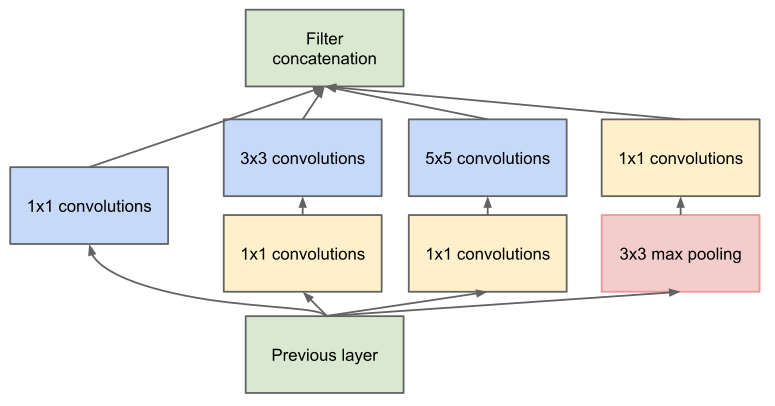
\includegraphics[width=0.8\columnwidth]{inception_block}
    \caption{Inception Block}
    \label{fig:inception_block}
\end{figure}

One of the focuses of GoogLeNet is to find the best convolution kernel size to avoid overfit problems and minimize the computational costs incurred when increasing the size of the Neural Network to improve performance. The fundamental way to solve both problems is to move from a fully connected architecture to an sparsely connected architecture, even within convolution. The Inception architecture was chosen after setting parameters and successfully demonstrated optimal performance.

According to Fig.\ref{fig:inception_block}, the inception block consists of 4 parallel paths. The first three paths use convolution layers with sizes 1x1, 3x3, and 5x5 to extract information of different spatial sizes. The two middle lanes perform 1×1 convolution on the input to reduce the number of channels, reducing model complexity. The fourth path uses a maximum 3x3 pooling layer, followed by a 1x1 convolution layer to change the number of channels. The four paths all use appropriate padding to provide input and output of the same height and width. Finally, the outputs along each line are combined along the channel dimensions and comprise block outputs.

\subsection{ResNet}
The ResNet paper is one of the most cited AI papers, and has been the foundation for neural networks with more than 1,000 layers. It was first introduced in 2015 by Kaiming He, Xiangyu Zhang, Shaoqing Ren and Jian Sun, but Despite its simplicity, the idea of residual connections is highly effective as it supports stable gradient propagation through the network. Instead of modeling $xl+1=F(xl)$, we model $xl+1=xl+F(xl)$ where $F$ is a non-linear mapping (usually a sequence of NN modules likes convolutions, activation functions, and normalizations) \cite{he2016deep}. If we do backpropagation on such residual connections, we obtain:

$$\frac{\partial x_{l+1}}{\partial x_{l}} = \mathbf{I} + \frac{\partial F(x_{l})}{\partial x_{l}}$$

The bias towards the identity matrix guarantees a stable gradient propagation being less effected by $F$ itself. There have been many variants of ResNet proposed, which mostly concern the function $F$, or operations applied on the sum. In this tutorial, we look at two of them: the original ResNet block, and the Pre-Activation ResNet block. We visually compare the blocks below.

\begin{figure}[!ht]
    \centering
    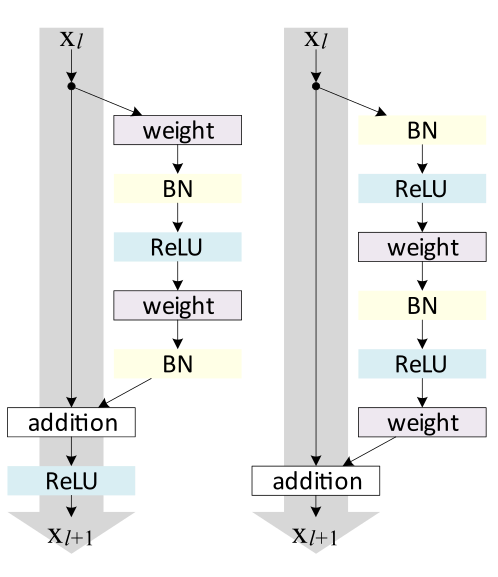
\includegraphics[width=0.8\columnwidth]{resnet_block}
    \caption{ResNet Block}
    \label{fig:resnet_block}
\end{figure}

The original ResNet block applies a non-linear activation function, usually ReLU, after the skip connection. In contrast, the pre-activation ResNet block applies the non-linearity at the beginning of F. Both have their advantages and disadvantages. For very deep network, however, the pre-activation ResNet has shown to perform better as the gradient flow is guaranteed to have the identity matrix as calculated above, and is not harmed by any non-linear activation applied to it. For comparison, in this notebook, we implement both ResNet types as shallow networks.

In Fig.\ref{fig:resnet_block} we can see that the original ResNet Block implements a non-linear activation function, usually ReLU, after the connection is passed. In contrast, the pre-activated ResNet block implements non-linearity at the beginning of F. Both have their advantages and disadvantages. However, for very deep networks, ResNet pre-activation has shown better performance because the gradient stream is guaranteed to have an identity matrix as calculated above, and is not harmed by the non-linear activation applied to it. For comparison, in this notebook, we implement both types of ResNet as a shallow network.

\subsection{DenseNet}
DenseNet is another architecture for enabling very deep neural networks and takes a slightly different perspective on residual connections. This architecture developed by Gao Huang, Zhuang Liu, and Laurens van der Marteen, instead of modeling the difference between layers, it considers residual connections as a possible way to reuse features across layers, removing any necessity to learn redundant feature maps. If we go deeper into the network, the model learns abstract features to recognize patterns \cite{huang2017densely}. However, some complex patterns consist of a combination of abstract features (e.g. hand, face, etc.), and low-level features (e.g. edges, basic color, etc.). To find these low-level features in the deep layers, standard CNNs have to learn copy such feature maps, which wastes a lot of parameter complexity. DenseNet provides an efficient way of reusing features by having each convolution depends on all previous input features, but add only a small amount of filters to it. See the figure below for an illustration.

\begin{figure}[!ht]
    \centering
    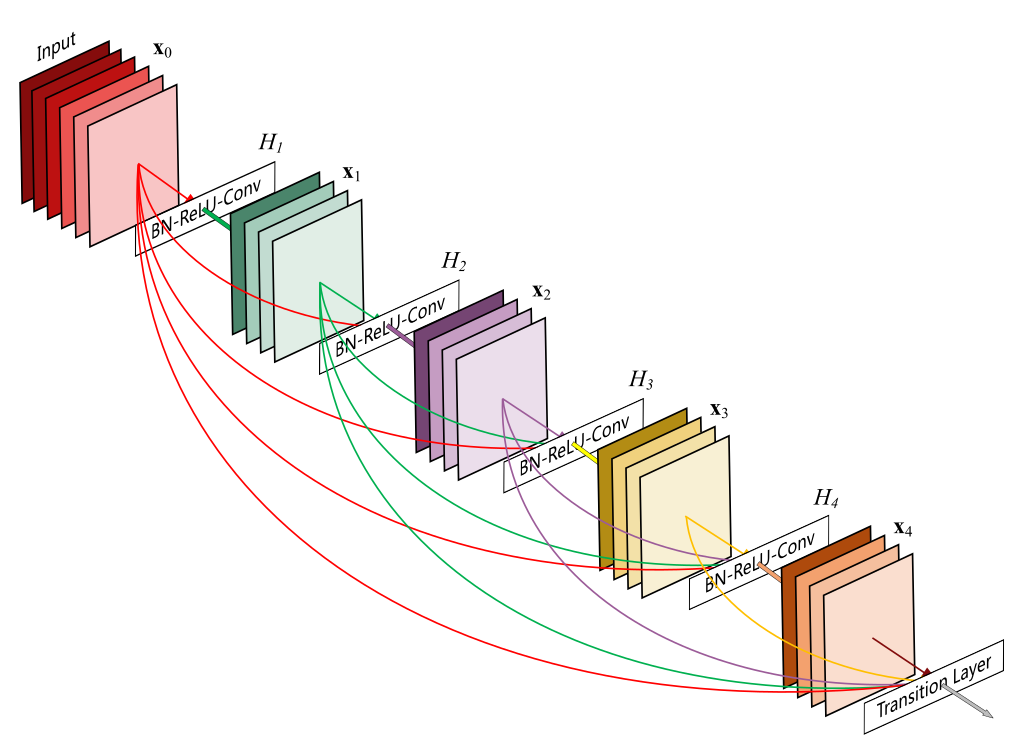
\includegraphics[width=0.8\columnwidth]{densenet_block}
    \caption{DenseNet Block}
    \label{fig:densenet_block}
\end{figure}

The last layer, called the transition layer, is responsible for reducing the dimensionality of the feature maps in height, width, and channel size. Although those technically break the identity backpropagation, there are only a few in a network so that it doesn't affect the gradient flow much.

We split the implementation of the layers in DenseNet into three parts: a DenseLayer, and a DenseBlock, and a TransitionLayer. The DenseLayer module implements a single layer inside a dense block. It applies a 1x1 convolution for dimensionality reduction with a subsequential 3x3 convolution. The output channels are concatenated to the originals and returned. Note that we apply the Batch Normalization as the first layer of each block. This allows slightly different activations for the same features to different layers, depending on what is needed.

\section{Research Methodology}

\subsection{Data Acquisition}
In this technical report, I used the CIFAR-10 dataset. CIFAR-10 is a dataset that contains a collection of images consisting of 60000 images divided into 10 classes where each class consists of 6000 images. Each data is 3 color images measuring 32x32. This dataset consists of 50000 training data and 10000 test data. The 10 classes contained in the CIFAR-10 dataset are airplane, automobile, cat, deer, dog, frog, horse, ship, truck \cite{krizhevsky2009cifar}. Before the dataset is used, it is necessary to normalize the dataset using the mean and std values of the dataset.

\subsection{Data Augmentaion}
Data augmentation is done in order to prevent overfitting. At this stage, two data augmentation processes will be carried out. First, the data augmentation process is carried out by flipping the image horizontally so that a new image with a different perspective is obtained. Generally, the flip process will not change the size of the image. The second augmentation process is resizing the image. The resizing process can change the scale and aspect ratio of the image. Therefore, after this process, the image will be cropped to a size of 32x32 so that it can then be inserted into the CNN model.

\subsection{Modelling}
To build the CNN model, I used three CNN architectures as previously mentioned, namely Inception, ResNet, and DenseNet. For the Inception model, the Adam optimizer is used with a learning rate of 0.001 and a weight decay of 0.0001. For the ResNet model, the activation functions used are ReLU and Stochastic Gradient Descent (SGD). In addition, the hyperparameters used are the learning rate used of 0.1, momentum of 0.9 and weight decay of 0.0001. The optimizer and hyperparameters apply to the 2 types of ResNet blocks used. For the ResNet architecture, 2 types of blocks will be used, namely the original ResNet Block and the Pre-Activation ResNet Block. The GoogleNet model in this study will use an activation function, namely ReLU. For the DenseNet model, the optimizer used is Adam and the activation function used is ReLU. In addition, the hyperparameter used is the learning rate used of 0.001 and the weight decay of 0.0001. In simple terms, the optimizer and hyperparameters used can be seen in the following table.

\begin{table}[H]
\centering
\begin{tabular}{l c c c c c} % The final bracket specifies the number of columns in the table along with left and right borders which are specified using vertical bars (|); each column can be left, right or center-justified using l, r or c. To specify a precise width, use p{width}, e.g. p{5cm}
\toprule % Top horizontal line
Model & Activation & Optimizer & Ir & Momentum & W. Decay \\ % Column names row
\midrule % In-table horizontal line
Inception & ReLU & Adam & 0.001 & - & 0.0001\\ % Content row 1
PreAct ResNet & ReLU & SGD & 0.1 & 0.9 & 0.0001\\ % Content row 2
ResNet & ReLU & SGD & 0.1 & 0.9 & 0.0001\\ % Content row 3
DenseNet & ReLU & Adam & 0.001 & - & 0.0001\\ % Content row 4
\midrule % In-table horizontal line
\midrule % In-table horizontal line
\end{tabular}
\smallskip
\caption{Model's Configuration} % Table caption, can be commented out if no caption is required
\label{tab:model_config} % A label for referencing this table elsewhere, references are used in text as \ref{label}
\end{table}

\section{Analysis and Interpretation}
In general, it can be seen that all models give a pretty good performance. From these results, it can be seen that Inception obtained the lowest performance in the validation accuracy and test accuracy sections of 90.40\% and 89.70\%, respectively. DenseNet provides slightly better performance when compared to Inception where there is an increase of 0.32\% in validation accuracy and 0.53\% in test accuracy. Finally, we can see that the performance of each ResNet model is able to outperform the Inception and DenseNet models where there is a difference of more than 1\% in the validation accuracy section and a difference of more than 1\% for test accuracy with Inception and a difference of close to 1\% when compared to DenseNet.

\begin{table}[H]
\centering
\begin{tabular}{l c c c c c} % The final bracket specifies the number of columns in the table along with left and right borders which are specified using vertical bars (|); each column can be left, right or center-justified using l, r or c. To specify a precise width, use p{width}, e.g. p{5cm}
\toprule % Top horizontal line
Model & Validation Accuracy & Test Accuracy & Number Parameters \\ % Column names row
\midrule % In-table horizontal line
Inception & 90.40\% & 89.70\% & 260,650 \\ % Content row 1
PreAct ResNet & 91.84\% & 91.06\% & 272,378 \\ % Content row 2
ResNet & 91.80\% & 91.07\% & 272,250 \\ % Content row 3
DenseNet & 90.72\% & 90.23\% & 239,146 \\ % Content row 4
\midrule % In-table horizontal line
\midrule % In-table horizontal line
\end{tabular}
\smallskip 
\caption{Model's Performance} % Table caption, can be commented out if no caption is required
\label{tab:model_perform} % A label for referencing this table elsewhere, references are used in text as \ref{label}
\end{table}

\section{Conclusions and Recommendations}
Based on the results obtained, ResNet provides the best performance when compared to the other 2 architectures. If we want to apply the architecture to more complex tasks with larger images, then we can see a big difference between GoogleNet and skip connection architectures like ResNet and DenseNet. Therefore, if we want to choose an architecture for a new task, then choosing the ResNet architecture is a good step considering its performance on the CIFAR-10 dataset.

% references
\bibliographystyle{plain} % We choose the "plain" reference style
\bibliography{refs} % Entries are in the refs.bib file

\end{document}


